\subsection{Geometry editor}
\label{sec:sf-geometry}

Geometry editor is a tool to create and edit geometry. Geometry consists of geometry objects. They are either lines or points. Geometry editor has following requirements.

\subsubsection{Functional Requirements}

\begin{enumerate}
	\item Geometry editor \textbf{shall} allow user to create, edit and delete points.
	\item Geometry editor \textbf{shall} allow user to create, edit and delete define point as inputPoint, Connector or bendPoint.
	\item Geometry editor \textbf{shall} allow user to create, edit and delete lines by using connectors and bendPoints.
	\item Geometry editor \textbf{shall} allow user to load and save geometry file.
	\item Geometry editor \textbf{shall} allow user to define labels for geometry objects.
	\item Geometry editor \textbf{shall} create unique IDs for geometry objects.
	\item Geometry editor \textbf{should} allow user to create parametric curved lines.
	\item Geometry editor \textbf{should} allow user to use undo and redo.
	\item Geometry editor \textbf{should} allow user to use copy, paste and cut geometry objects.
	\item Geometry editor \textbf{should} have a Graphical User Interface.
	\begin{enumerate}
		\item Geometry editor \textbf{should} have drag and drop interface.
		\item Geometry editor \textbf{should} enable editing of geometries with a text input.
		\item It \textbf{would be nice} if the geometry editor allows user to create different kinds of parametric curved lines, such as Catmull-rom spline and Bézier-curves.
		\item It \textbf{would be nice} if the geometry editor allows user to zoom and pan the geometry canvas.
		\item It \textbf{would be nice} if the geometry editor allows user select multiple geometry objects simultaneously.
		\item It \textbf{would be nice} if the geometry editor allows user to load multiple geometries on same canvas.
		\item It \textbf{would be nice} if the geometry editor allows user select multiple geometry objects simultaneously.
		\item It \textbf{would be nice} if the geometry editor allows user to rotate and scale geometry objects.
		\item It \textbf{would be nice} if the geometry editor allows user to toggle visibility of geometry objects while using geometry editor.
	\end{enumerate}
	\item It \textbf{would be nice} if you could specify a Petri ned model from which the geometry is being specified from and it is validated.
\end{enumerate}

\subsubsection{Use cases}

The uses of geometry editor is summed up in the use case diagram in Figure~\ref{fig:use-cases-geometry-editor}.

\begin{figure}[htp]
\begin{center}
  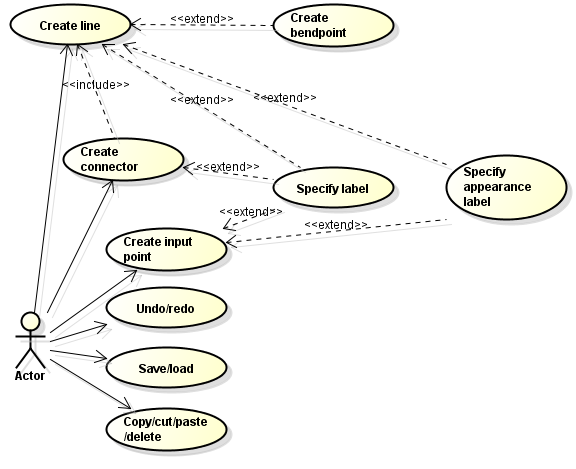
\includegraphics[width=0.8\textwidth]{image/uc-geometry.png}
  \caption{Use cases for the Geometry editor}
  \label{fig:use-cases-geometry-editor}
\end{center}
\end{figure}